\documentclass[preprint]{aastex}
%\documentclass{emulateapj}


% has to be before amssymb it seems
%\usepackage{color,hyperref}
%\definecolor{linkcolor}{rgb}{0,0,0.5}
%\hypersetup{colorlinks=true,linkcolor=linkcolor,citecolor=linkcolor,
%            filecolor=linkcolor,urlcolor=linkcolor}
%\usepackage{amssymb,amsmath}

\usepackage{color}
\usepackage{url}
\usepackage{graphicx}
\graphicspath{{figures/}}

% For Python code
\usepackage{listings}
\definecolor{lbcolor}{rgb}{0.9,0.9,0.9}
\lstset{language=Python,
        basicstyle=\footnotesize\ttfamily,
        showspaces=false,
        showstringspaces=false,
        tabsize=2,
        breaklines=false,
        breakatwhitespace=true,
        identifierstyle=\ttfamily,
        keywordstyle=\bfseries\color[rgb]{0.133,0.545,0.133},
        commentstyle=\color[rgb]{0.133,0.545,0.133},
        stringstyle=\color[rgb]{0.627,0.126,0.941},
    }

% Draft watermark:
%\usepackage{draftwatermark}
%\SetWatermarkLightness{0.9}
%\SetWatermarkScale{4}

\usepackage{amsmath}
\DeclareMathOperator{\sinc}{sinc}
\DeclareMathOperator{\III}{III}

% Some macros
\newcommand{\todo}[1]{{\color{red} [TODO: #1]}}
\newcommand{\foreign}[1]{{\it #1}}

\newcommand{\apriori}{\foreign{a priori}}
\newcommand{\adhoc}{\foreign{ad hoc}}
\newcommand{\etal}{\foreign{et\,al.}}
\newcommand{\etc}{\foreign{etc.}}

\newcommand{\Fig}[1]{Figure~\ref{fig:#1}}
\newcommand{\fig}[1]{Figure~\ref{fig:#1}}
\newcommand{\figs}[2]{Figures~\ref{fig:#1}-\ref{fig:#2}}
\newcommand{\figlabel}[1]{\label{fig:#1}}
\newcommand{\Eq}[1]{Equation~(\ref{eq:#1})}
\newcommand{\eq}[1]{\Eq{#1}}
\newcommand{\eqs}[2]{Equations~(\ref{eq:#1})-(\ref{eq:#2})}
\newcommand{\eqlabel}[1]{\label{eq:#1}}
\newcommand{\Sect}[1]{Section~\ref{sect:#1}}
\newcommand{\sect}[1]{\Sect{#1}}
\newcommand{\sects}[1]{Sections~#1}
\newcommand{\App}[1]{Appendix~\ref{sect:#1}}
\newcommand{\app}[1]{\App{#1}}
\newcommand{\sectlabel}[1]{\label{sect:#1}}

\usepackage[normalem]{ulem}
\newcommand{\new}[1]{{\color{red} #1}}
\newcommand{\old}[1]{{\sout{#1}}}


\begin{document}

\title{Understanding the Lomb-Scargle Periodogram}

\newcommand{\escience}{*}
\newcommand{\uwastro}{+}
\author{Jacob T. VanderPlas\altaffilmark{\escience}}
\altaffiltext{\escience}{eScience Institute, University of Washington}


\begin{abstract}
This paper gives an introduction to the practical aspects of the use of Lomb-Scargle periodograms and related algorithms to detect periodic signals.
Rather than a rigorous mathematical treatment, the goal of this paper is to build intuition about what assumptions are baked into any periodogram computation.
We discuss... and ... and ...
\end{abstract}

\keywords{
    methods: data analysis ---
    methods: statistical
}

\section{Introduction}
\sectlabel{introduction}

\begin{figure}[ht]
\centering
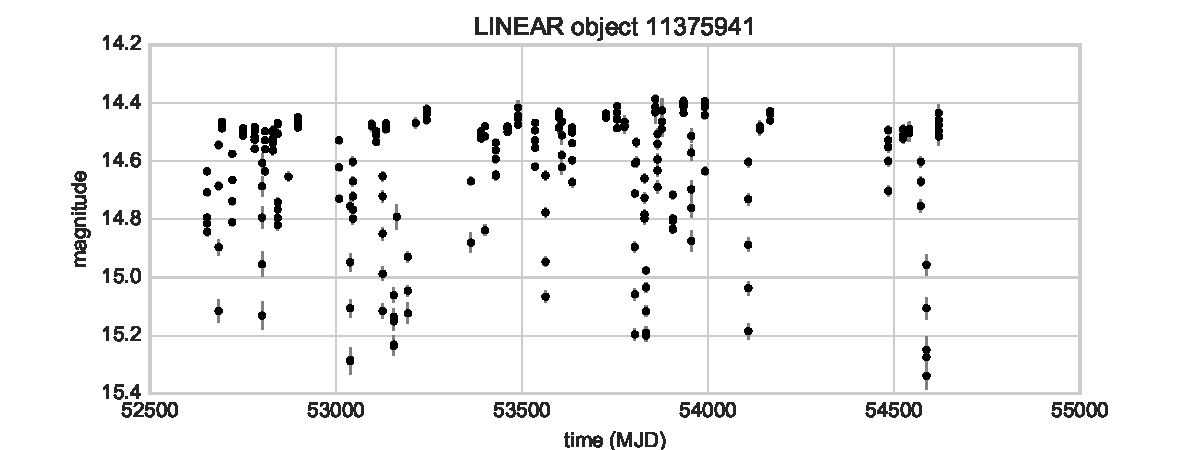
\includegraphics[width=\textwidth]{fig01_LINEAR_data}
\caption{Observed light curve from LINEAR object ID 11375941. Uncertainties
  are indicated by the gray errorbars on each point.
  \figlabel{LINEAR-data}
}
\end{figure}


\begin{figure}[ht]
\centering
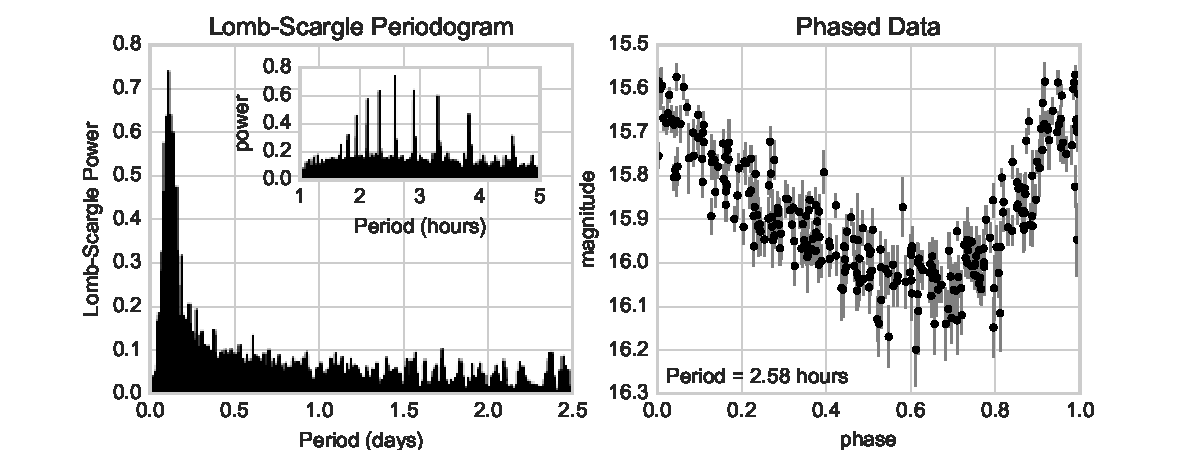
\includegraphics[width=\textwidth]{fig02_LINEAR_PSD}
\caption{{\it Left panel:} the Lomb-Scargle periodogram computed from the data
    shown in \fig{LINEAR-data}, with an inset detailing the region near the peak.
    {\it Right panel:} the input data in \fig{LINEAR-data}, folded over the
    detected 2.58-hour period to show the coherent periodic variability.
    For more discussion of this data, see \citep{LINEAR3}.
    \figlabel{LINEAR-power}
}
\end{figure}

The Lomb-Scargle periodogram \citep{Lomb76, Scargle82}
is a well-known algorithm for detecting periodicity
in unevenly-sampled time-series, particularly within the astronomy community.
For example, consider the data shown in \fig{LINEAR-data}.
This is an irregularly-sampled timeseries showing a single object from the
LINEAR survey \citep{LINEAR1, LINEAR3}, with magnitude measured 280 times over
the course of five and a half years\footnote{
  Python code to reproduce \fig{LINEAR-data}, as well as all other figures
  in this manuscript, is available at 
  \url{http://github.com/jakevdp/PracticalLombScargle/}}.

By eye, it is clear that the brightness of the object varies in time with a range spanning approximately 0.8 magnitudes, but what is not immediately clear is that this variation is periodic in time.
The Lomb-Scargle periodogram is a method that allows efficient computation of a Fourier-like power spectrum from such unevenly-sampled data, resulting in an intuitive means of determining the period of oscillation.

The left panel of \fig{LINEAR-power} shows the Lomb-Scargle periodogram computed for the data in \fig{LINEAR-data}.
Computing the Lomb-Scargle periodogram for the data gives us a measure of the
power as a function of period of oscillation (\fig{LINEAR-power}, left), from
which we can determine the period of oscillation of approximately 2.58 hours.
The right panel of \fig{LINEAR-power} shows a folded visualization of
the same data as \fig{LINEAR-data} -- i.e.{} plotted as a function of phase
rather than time.\footnote{
    The periodogram in \fig{LINEAR-power} was computed using
    {\tt astropy.stats.LombScargle}
    from the AstroPy project; see \url{http://astropy.org/}.
}

Often this is exactly how the Lomb-Scargle periodogram is presented: as a clean, well-defined procedure to detect the periodic component in an unevenly-sampled dataset.
In practice, however, there are a number of subtle issues that must be considered when applying a Lomb-Scargle analysis to real-world datasets, and I have found that these are rarely presented together at an introductory level.
Here are a few questions in particular that we might wish to ask about the results in \fig{LINEAR-power}:
\begin{enumerate}
  \item What is the source of the multiple peaks revealed by the Lomb-Scargle Periodogram?
  \item What is a suitable range of frequencies to search for a given dataset?
  \item What is the Nyquist frequency for this type of analysis?
  \item How should we choose the spacing of the frequency grid for our periodogram?
  \item How should we understand the uncertainty of the computed frequency?
  \item What assumptions is the Lomb-Scargle periodogram making about the signal?
\end{enumerate}
Questions like these are discussed in various textbooks and review papers, but I have not come across any concise reference that discusses such questions in depth.
This paper seeks to fill that gap, and provide a practical, semi-technical guide to the effective use of the Lomb-Scargle method of periodic analysis.
This paper does not seek a complete or rigorous treatment of the mathematics involved, but rather seeks to develop the intuition of {\it how} to think about the issues involved.


\section{Background: the Continuous Fourier Transform}

In order to understand how we should interpret the Lomb-Scargle periodogram, we will first briefly step back and review the subject of Fourier analysis of continuous signals.
Consider a continuously-defined signal $g(t)$.
Its Fourier transform is given by the following integral:
\begin{equation}
    \hat{g}(f) \equiv \int_{-\infty}^\infty g(t) e^{-2\pi i f t} dt
    \eqlabel{FT-def}
\end{equation}
The inverse relationship is given by:
\begin{equation}
    g(t) \equiv \int_{-\infty}^\infty \hat{g}(f) e^{+2\pi i f t} df
    \eqlabel{IFT-def}
\end{equation}
For convenience we will also define the Fourier transform operator
$\mathcal{F}$, such that
\begin{eqnarray}
    \mathcal{F}\{g\} &=& \hat{g} \\
    \mathcal{F}^{-1}\{\hat{g}\} &=& g
\end{eqnarray}
As a further shorthand, we'll sometimes use a double arrow to denote a Fourier
pair; for example
\begin{equation}
  g(x) \Longleftrightarrow \hat{g}(f).
\end{equation}

\subsection{Properties of the Fourier Transform}

The continuous Fourier transform has a number of useful properties that we will make use of in our discussion.

\begin{description}
   \item[The Fourier transform is a linear operation.]
     That is, for any constant $A$ and any functions $f$ and $g$, we can write
     \begin{eqnarray}
       \mathcal{F}\{f(t) + g(t)\} &=& \mathcal{F}\{f(t)\} + \mathcal{F}\{g(t)\}\nonumber\\
       \mathcal{F}\{A f(t)\} &=& A\mathcal{F}\{f(t)\}
     \end{eqnarray}
     which follows from the linearity of the Fourier integral.

   \item[The Fourier transform of sinusoid with frequency $f_0$ is a sum of delta functions at $\pm f_0$.]
     Given the integral definition of the Dirac delta function, it is straightforward to show that
     \begin{equation}
       \mathcal{F}\{e^{2\pi f_0 t}\} = \delta(f - f_0).
       \eqlabel{delta-FT}
     \end{equation}
     Euler's formula shows how such a complex exponential
     can be expressed in terms of sines and cosines:
     \begin{equation}
       e^{2\pi f_0 t} = \cos(2\pi f_0 t) + i\sin(2\pi f_0 t).
       \eqlabel{Euler-formula}
     \end{equation}
     Using the linearity of the Fourier transform, we can take these identites
     and derive the following identities:
     \begin{eqnarray}
       \mathcal{F}\{\cos(2\pi f_0 t)\} &=& \frac{1}{2}\left[\delta(f - f_0) + \delta(f + f_0)\right]\nonumber\\
       \mathcal{F}\{\sin(2\pi f_0 t)\} &=& \frac{1}{2i}\left[\delta(f - f_0) - \delta(f + f_0)\right].
     \end{eqnarray}
     In other words, a sinusoidal signal with frequency $f_0$ has a Fourier transform consisting of a weighted sum of delta functions at $\pm f_0$.

   \item[A time-shift imparts a phase in the Fourier transform.]
     Given a well-behaved function $g(t)$ we can use a transformation of
     variables to derive the following identity:
     \begin{equation}
       \mathcal{F}\{g(t - t_0)\} = \mathcal{F}\{g(t)\} e^{-2\pi i ft_0}
     \end{equation}
     The key observation here is that the time-shift does not change the
     amplitude of the resulting transform, but only the phase.
\end{description}
These properties taken together make the Fourier transform quite useful for the study of periodic signals.
The linearity of the transform means that any signal made up of a sum of periodic components will have a Fourier transform consisting of a sum of delta functions at those frequencies: that is, the Fourier transform is a {\it direct} measure of the periodic content of a function.

Further, if we compute the squared amplitude of the resulting transform, we can both do away with complex components and remove the phase imparted by any time offsets; this squared amplitude is usually known as the {\it Power Spectrum}:
\begin{equation}
  \mathcal{P}\{g\} \equiv \left|\mathcal{F}\{g\}\right|^2
  \eqlabel{power-spectrum}
\end{equation}
The power spectrum of a function is a positive real-valued function of $f$ that quantifies the contribution of each frequency $f$ to the total signal.

\subsection{Some Useful Fourier Pairs}

\begin{figure}[ht]
\centering
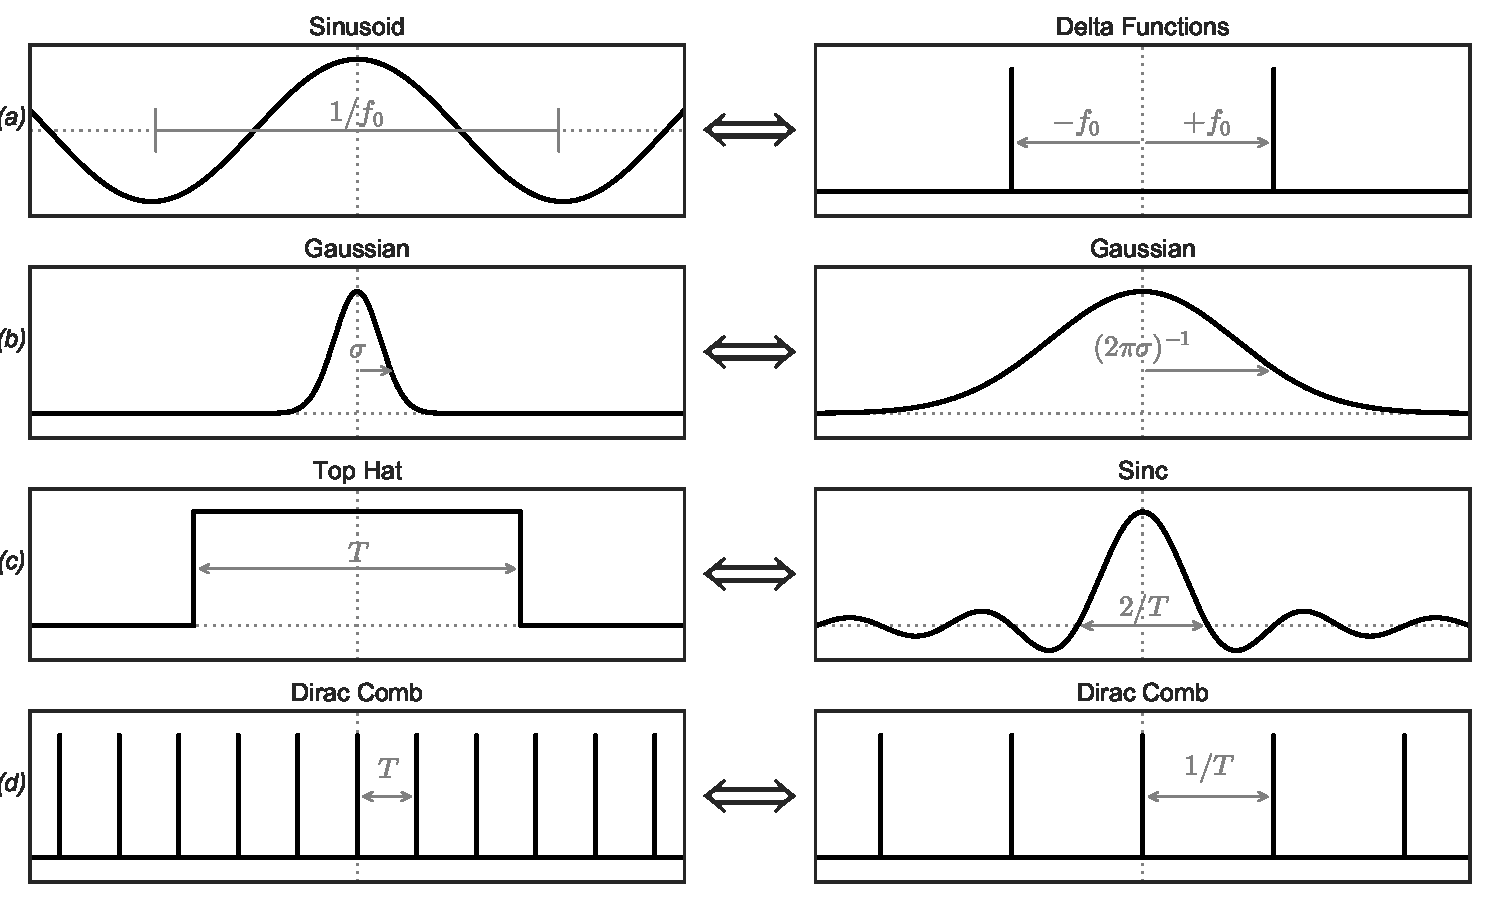
\includegraphics[width=\textwidth]{fig03_Fourier_pairs}
\caption{Visualization of important Fourier pairs.\figlabel{fourier-pairs}}
\end{figure}

We have already discussed that the Fourier transform of a complex exponential is a single delta function.
This is just one of many ``Fourier Pairs'' to keep in mind as we progress to understanding the Lomb-Scargle Periodogram.
We list a few more important pairs here (see \Fig{fourier-pairs} for a visual representation of the following pairs):


\begin{description}
  \item[The Fourier transform of a sinusoid is a pair of Delta functions.]
    (See \fig{fourier-pairs}{\it a})
    \begin{equation}
      \mathcal{F}\{\cos(2\pi f_0 t)\} = \frac{1}{2}\left[\delta(f-f_0) + \delta(f+f_0)\right]
    \end{equation}
    We saw this above, but repeat it here for completeness.

   \item[The Fourier transform of a Gaussian is a Gaussian.]
    (See \fig{fourier-pairs}{\it b})
     \begin{equation}
       \mathcal{F}\{{\rm N}(t; \sigma)\} = \frac{1}{\sqrt{2\pi\sigma^2}}{\rm N}\left(f;\frac{1}{2\pi\sigma}\right)
     \end{equation}
     The Gaussian function ${\rm N}(t, \sigma)$ is given by
     \begin{equation}
       {\rm N}(t; \sigma) \equiv \frac{1}{\sqrt{2\pi\sigma^2}}e^{-t^2/(2\sigma^2)}
     \end{equation}

  \item[The Fourier transform of a tophat function is a sinc function.]
    (See \fig{fourier-pairs}{\it c})
    \begin{equation}
      \mathcal{F}\{\Pi_T(t)\} = \sinc(f T)
    \end{equation}
    The tophat function, $\Pi_T(t)$, is a normalized symmetric function that
    is uniform within a range given by $T$, and zero elsewhere:
    \begin{equation}
      \Pi_T(t)  \equiv \left\{
      \begin{array}{ll}
        1 / T, & |t| \le T / 2 \\
        0,     & |t| > T / 2
      \end{array}
      \right.
    \end{equation}
    The sinc function is given by the standard definition:
    \begin{equation}
      \sinc(x) \equiv \frac{\sin(\pi x)}{\pi x}
    \end{equation}

  \item[The Fourier transform of a Dirac comb is a Dirac comb.]
    (See \fig{fourier-pairs}{\it d})
    \begin{equation}
      \mathcal{F}\{\III_T(t)\} = \frac{1}{T}\III_{1/T}(f)
    \end{equation}
    The Dirac comb, $\III_T(t)$, is an infinite sequence of Dirac delta functions placed at even intervals of size $T$:
    \begin{equation}
      \III_T(t) \equiv \sum_{n=-\infty}^\infty \delta(t - nT)
      \eqlabel{dirac-comb}
    \end{equation}
\end{description}
The key observation in each of these Fourier pairs is the reciprocity
of scales between a function and its Fourier transform:
that is, a function with a characteristic scale $T$ will in general
have a Fourier transform with characteristic scale of $1/T$.
This feature will turn out to be very important as we push further in
understanding the Lomb-Scargle Periodogram.


\subsection{The Convolution Theorem}

A final property of the Fourier transform that we will discuss here is its
ability to convert convolutions into point-wise products.
A convolution of two functions, usually denoted with a $\ast$, is defined
as follows:
\begin{equation}
  [f \ast g](t) = \int_{-\infty}^\infty f(\tau)g(t - \tau) d\tau
  \eqlabel{convolution-definition}
\end{equation}
From the definition, it is clear that a convolution amounts to ``sliding'' one
function past the other.
Such an operation is commonly used, for example, in smoothing a function,
as visualized in \Fig{convolution} for a tophat-shaped smoothing window.

\begin{figure}[ht]
  \centering
  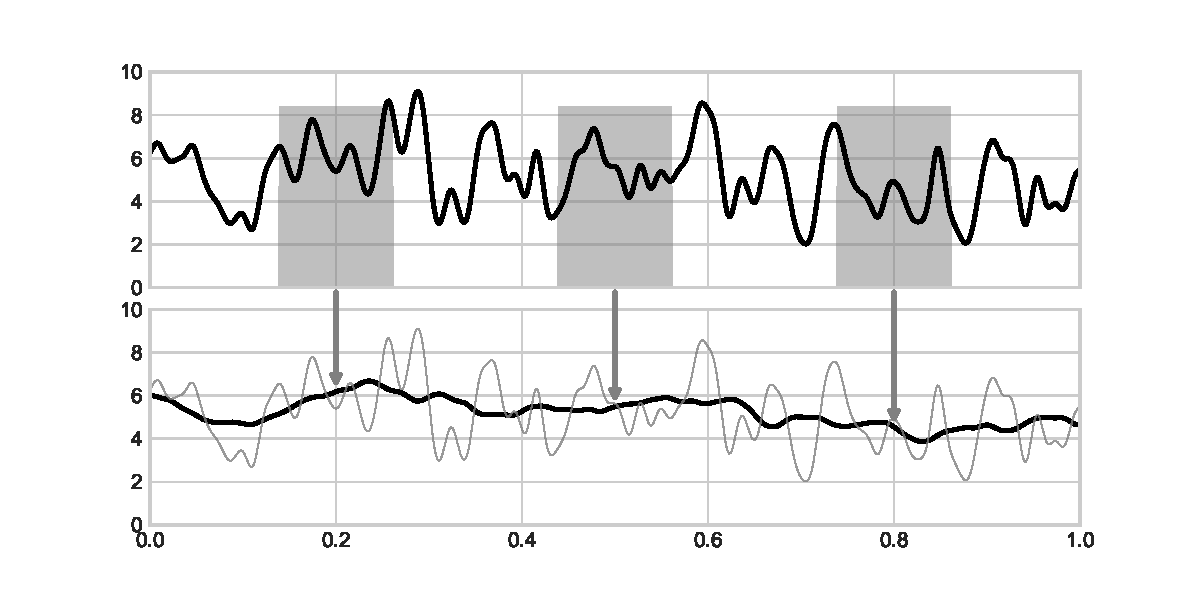
\includegraphics[width=\textwidth]{fig04_Convolution_Diagram}
  \caption{Visualization of a convolution between a continuous signal and a tophat smoothing kernel.
    The normalized tophat-shaped window function slides across the domain (upper panel),
    such that at each point the mean of the values within the window are
    used to compute the smoothed function (lower panel).
    \figlabel{convolution}}
\end{figure}

Given this definition of a convolution, it can be shown that the Fourier transform of a convolution is the point-wise product of the Fourier transforms:
\begin{equation}
  \mathcal{F}\{f \ast g\} = \mathcal{F}\{f\} \cdot \mathcal{F}\{g\}
  \eqlabel{convolution-theorem}
\end{equation}
In practice, this is a much more efficient means of computing the convolution
than to directly solve at each time $t$ the integral over $\tau$ that appears
in \eq{convolution-definition}.
This result in \eq{convolution-theorem} is known as the
{\it convolution theorem}, and is illustrated in \fig{convolution-theorem}.
\begin{figure}[ht]
  \centering
  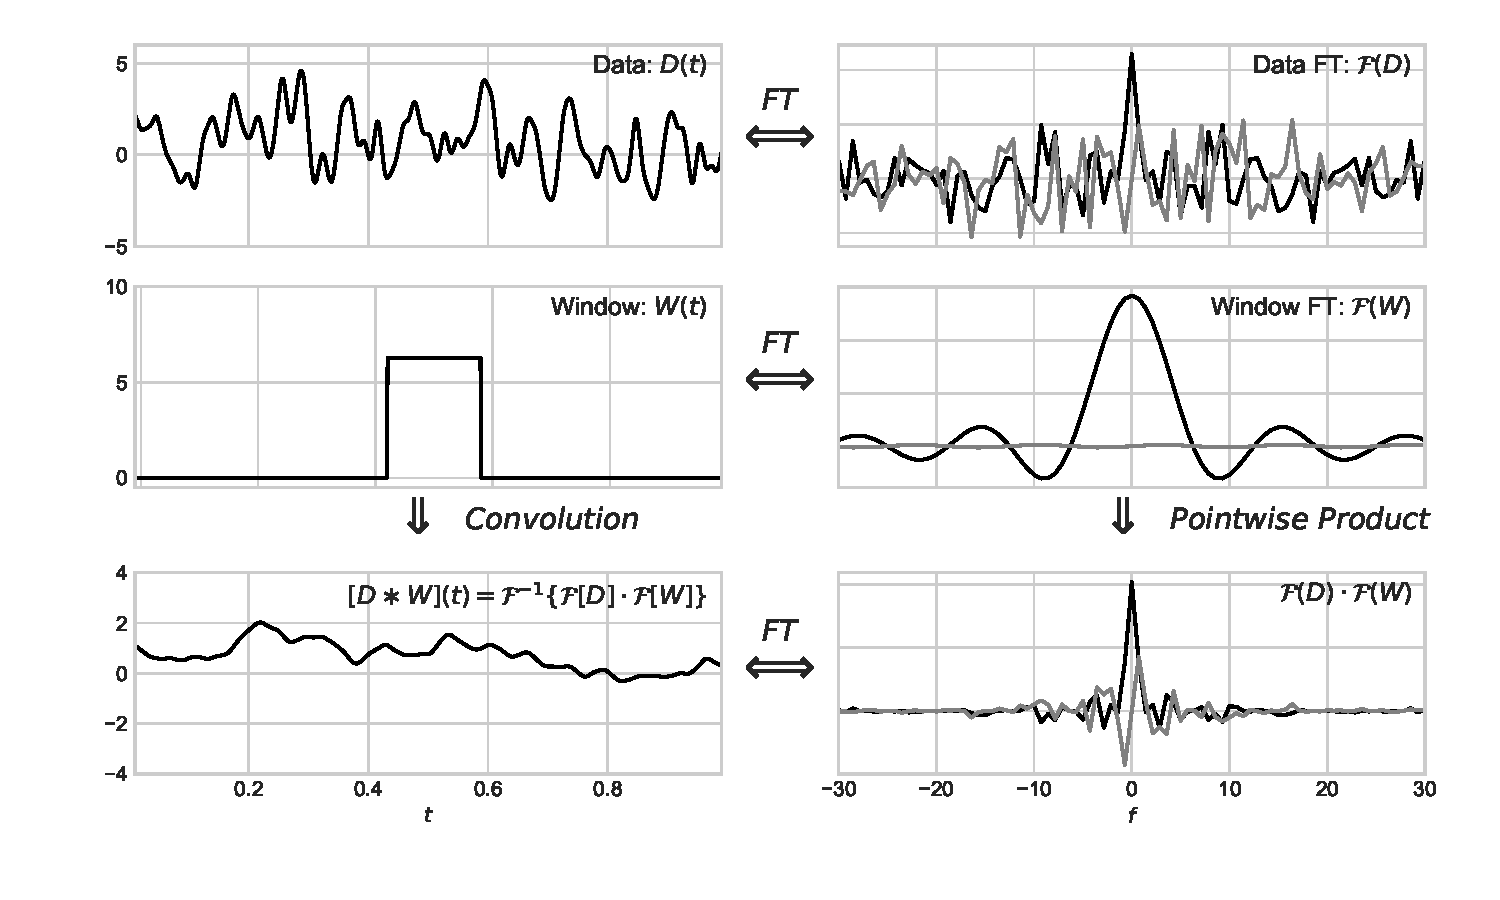
\includegraphics[width=\textwidth]{fig05_Convolution_Theorem}
  \caption{Visualization of the convolution theorem (\eq{convolution-theorem}).
    The key is that the Fourier transform of
    a convolution is the pointwise product of the two Fourier transforms.
    In the right panels, the black and gray lines represent the real and
    imaginary part of the transform, respectively.
    \figlabel{convolution-theorem}}
\end{figure}
When thinking about frequency components of time-domain measurements, this
property of the Fourier transform becomes essential, as we will see.

An important corrollary is that the Fourier transform of a product is a convolution of the two transforms:
\begin{equation}
  \mathcal{F}\{f \cdot g\} = \mathcal{F}\{f\} \ast \mathcal{F}\{g\}
  \eqlabel{convolution-theorem-inverse}
\end{equation}
We will explore the impact of this in the next section.

\section{Window Functions: From Idealized to Real-world signals}
In a typical observational setting, we will be observing some small part of
a larger time-varying signal.
For example, if you have a very long signal that you measure for a finite
amount of time, your measurement is a point-wise product between the true
signal and a suitable tophat function describing your measurement process.
If you have a continuous signal that you measure at regular intervals, your
measurement is a point-wise product between the true signal and an appropriate
Dirac comb describing your measurement process.
From what we learned about the convolution theorem in the previous section, it
is clear that {\it the measured Fourier transform will be the true transform
convolved with the transform of the obverving window}.
This has some interesting consequences, as we shall see.

\subsection{Effect of a Tophat Window}
First, let's consider the case of observing a continuous periodic signal over
a limited span of time, as illustrated in \Fig{tophat-window}.
Here we consider a periodic function made up of three frequency components, observed within a 10-unit time window.
The observed signal in this case can be thought of as a pointwise product of an infinite periodic signal, and a tophat window function.
Using \eq{convolution-theorem-inverse}, we see that the Fourier transform of
this function is equivalent to the convolution of the Fourier transforms of each component, which are a set of delta functions and a sinc function, respectively.
For a purely periodic signal, this convolution has the effect of broadening the delta functions representing the signal, turning each of them into a shifted sinc function.
Because of the inverse relationship between the width of the window and the width of its transform (see \Fig{fourier-pairs}), it follows that a wider observing window leads to proportionally less spread in the Fourier transform of the observed function.

\begin{figure}[ht]
  \centering
  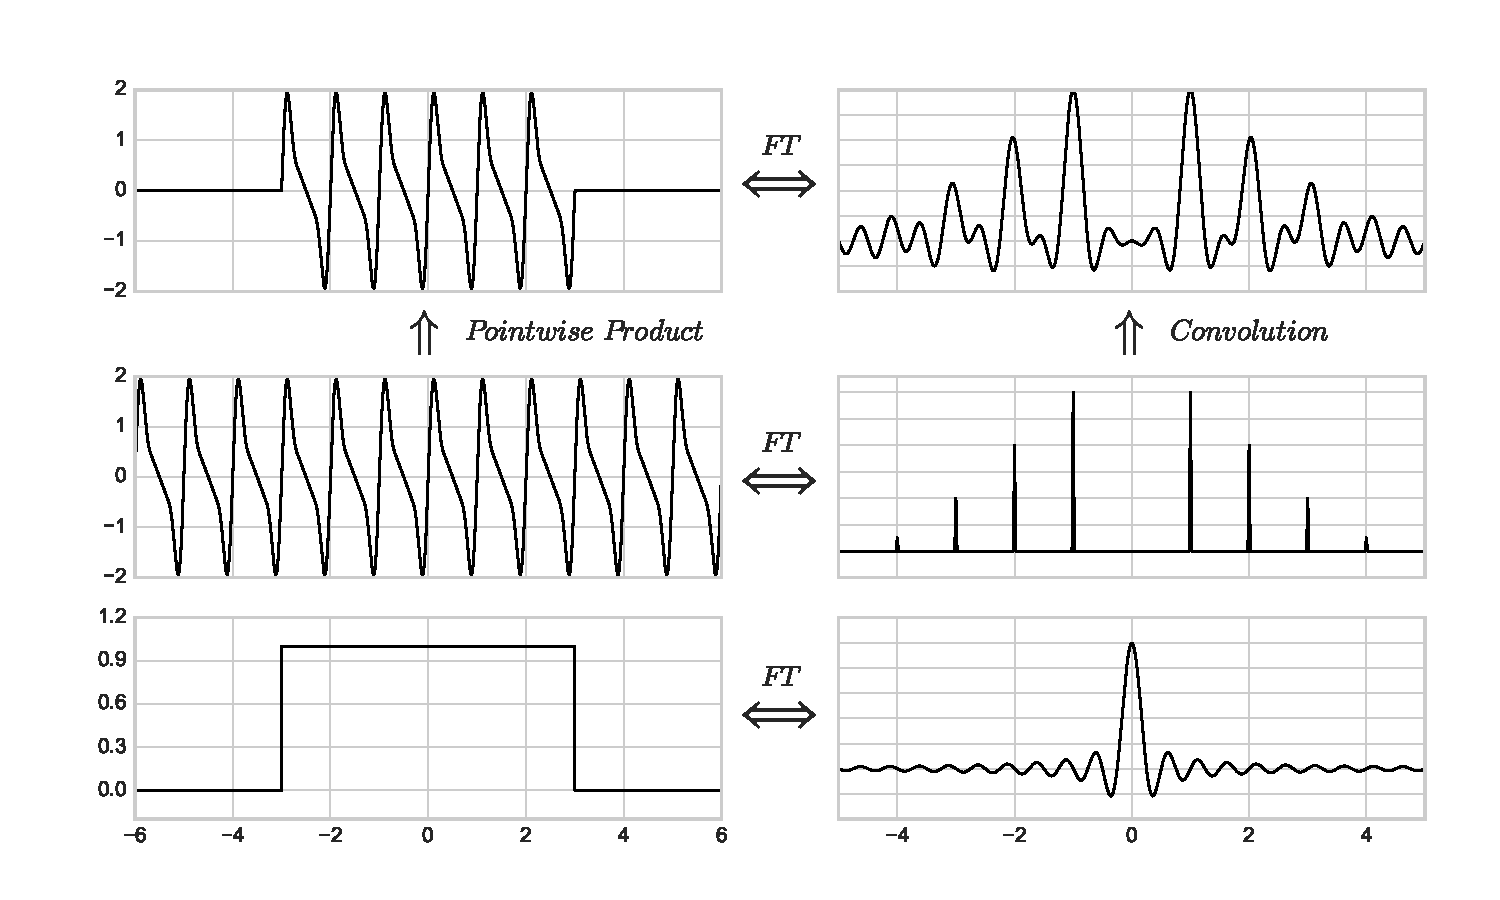
\includegraphics[width=\textwidth]{fig06_Tophat_Window}
  \caption{Visualization of the effect on the Fourier transform of a
    tophat-shaped observing window (i.e., a continuous signal observed
    fully, but only within a finite range of time). The observed Fourier
    transform is a convolution of the true transform (here a series of Delta
    functions) and the window transform (here a narrow sinc function).
    \figlabel{tophat-window}}
\end{figure}

\subsection{The Dirac Comb and the Discrete Fourier Transform}
Another window function that commonly arises is when a continuous signal is
sampled instantaneously at regular intervals.
Such an observation is, in effect, a point-wise product between the true
underlying signal and a Dirac comb with the $T$ parameter matching the spacing
of the observations; this is illustrated in \fig{comb-window-1}.

\begin{figure}[ht]
  \centering
  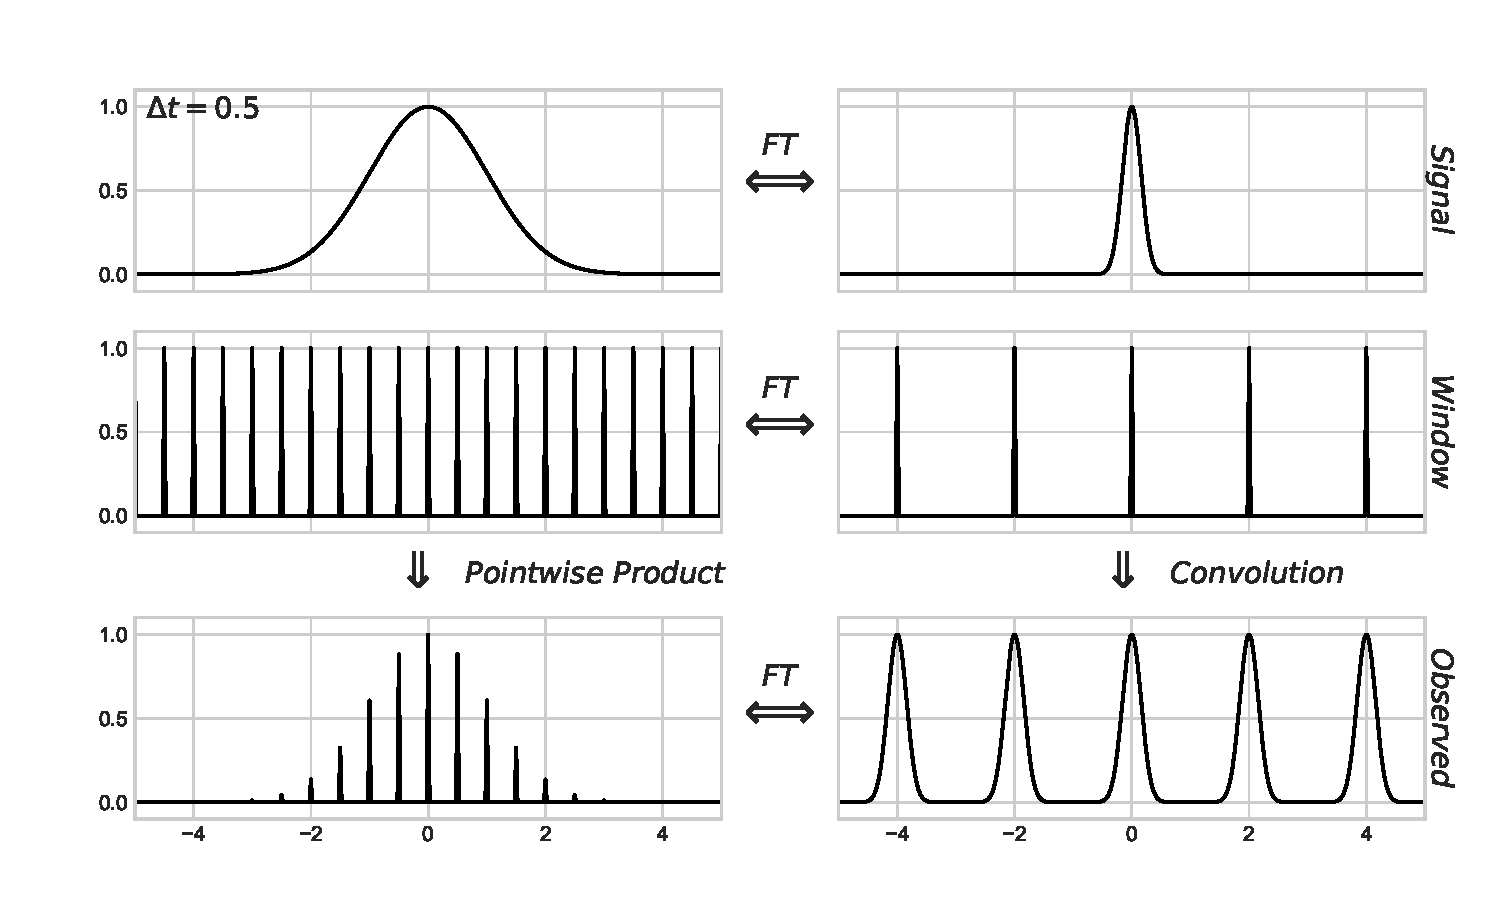
\includegraphics[width=\textwidth]{fig07_comb_window_1}
  \caption{Visualization of the effect on the Fourier transform of a
    Dirac Comb observing window (i.e., a long string of evenly-spaced
    discrete observations). The observed Fourier
    transform is a convolution of the true transform (here a localized
    Gaussian) and the window transform (here another Dirac comb).
    \figlabel{comb-window-1}}
\end{figure}

Interestingly, because the Fourier transform of a Dirac comb is another Dirac
comb, the effect of such an observing window is to create a long sequence
of aliases with a spacing of $1/T$.
With this in mind, we can be assured in this case that evaluating the
transform in the range $(2T)^{-1} \le f < (2T)^{-1}$ is sufficient to capture
all the available frequency information:
the signal outside that range is a sequence of identical aliases of
what lies in that range.
In fact, due to the nature of the aliasing, it is in fact sufficient to
compute the transform in {\it any} range of width $1/T$, and it is often
convenient to instead use the range $0 \le f < 1/T$.

\subsubsection{The Nyquist Limit}
\sectlabel{nyquist}

The example in \fig{comb-window-1} is somewhat of a best-case scenario, because
the true Fourier transform values lie entirely in a range of width $1/T$.
If we change the sampling rate so that this is no longer the case, we will
have a situation similar to that in \fig{comb-window-2}.
With a lower sampling rate, the signal transform no longer fits within the
frequency window, and the true Fourier transform {\it cannot be recovered}
from the observed transform.

This implies that if we have a regularly-sampled function with a sampling
rate of of $f_0 = 1/T$, we can only fully recover the freuqency information
if the signal is {\it band-limited} between frequencies $\pm f_0/2$.
This is one way to motivate the famous Nyquist sampling limit, which says
that to fully represent the frequency content of a ``band-limited signal''
with all Fourier power in the range $\pm B$, we must sample the data with a
rate of at least $2B$.

\begin{figure}[ht]
  \centering
  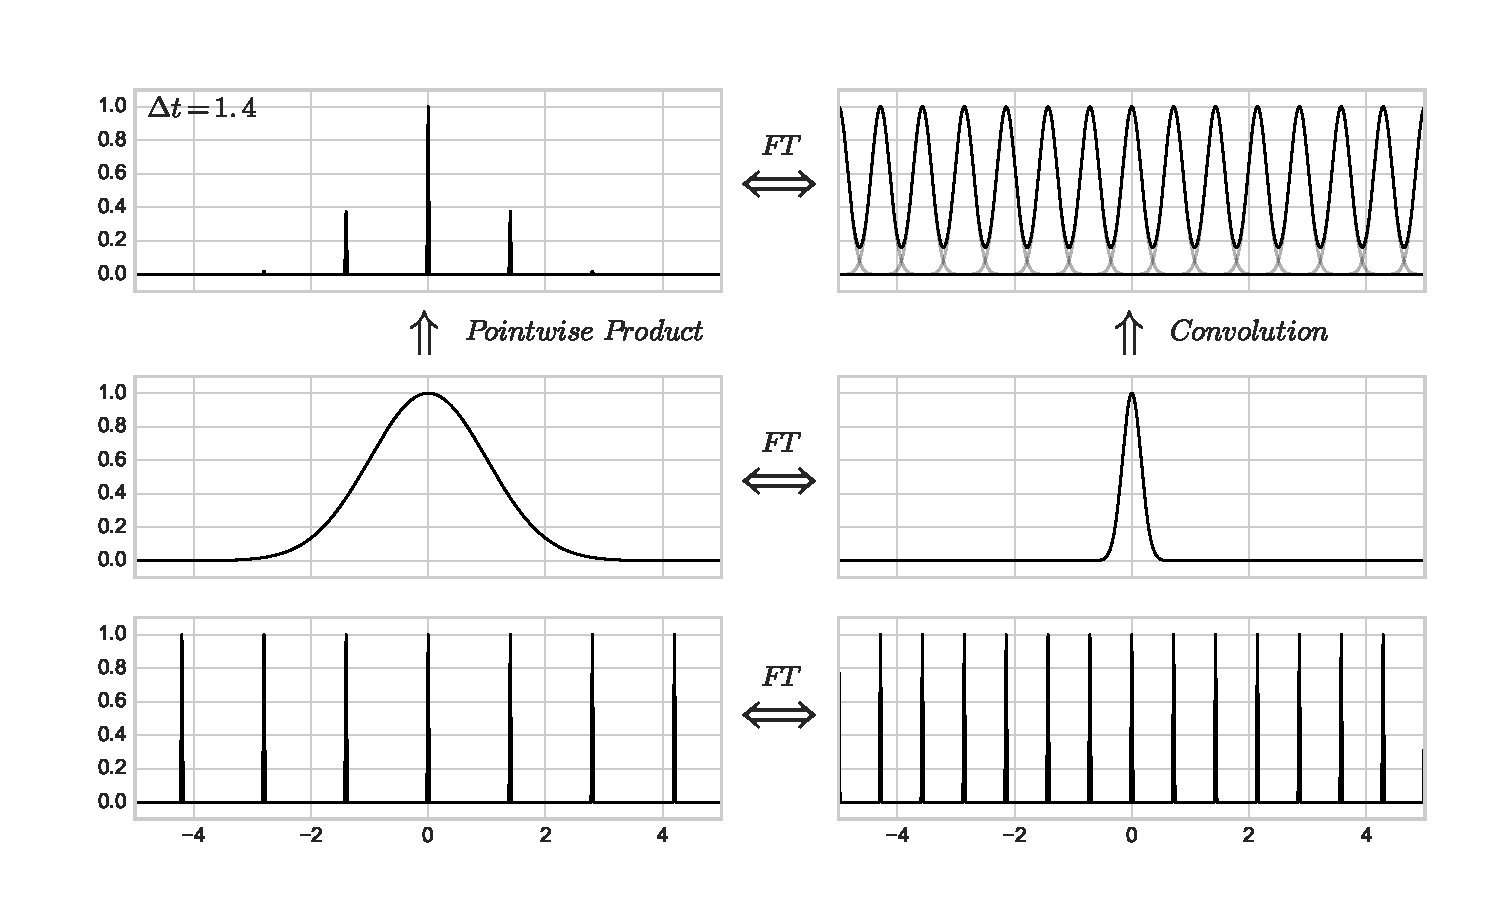
\includegraphics[width=\textwidth]{fig08_comb_window_2}
  \caption{Repeating the visualization from \fig{comb-window-1}, but here with
    a lower sampling rate. The result is that the Fourier transform of the
    window function (lower left) has spacing narrower than the Fourier transform
    of the signal (middle left), meaning the observed Fourier transform has
    aliasing of signals, such that not all frequency information can be
    recovered.
    \figlabel{comb-window-2}}
\end{figure}

\subsubsection{The Discrete Fourier Transform}
For regularly-spaced observations defined by a Dirac comb, the delta functions
serve to collapse the Fourier integral into a sum over periodic components.
Suppose we have a true (infinitely long and continuous) signal $g(t)$, but
we observe it only at a regular grid with spacing $T$. In this case, our
observed signal is $g_{obs} = g(t) \III_T(t)$ and its Fourier transform is
\begin{equation}
  \hat{g}_{obs}(f) = \sum_{n=-\infty}^\infty g(nT) e^{-2\pi i f n T},
\end{equation}
which follows directly from \eq{FT-def} and \eq{dirac-comb}.

In the real world, however, we will not have an infinite number of observations,
but rather a finite number of samples $N$.
We can choose the coordinate system appropriately and define
$g_n \equiv g(nT)$ to write
\begin{equation}
  \hat{g}_{obs}(f) = \sum_{n=0}^N g_n e^{-2\pi i f n T}
  \eqlabel{DFT-f}
\end{equation}
From the arguments around Nyquist aliasing, we know that the only relevant
frequency range is from $0 \le f \le 1/T$, and so we can define $N$
evenly-spaced frequencies with $\Delta f = 1 / (NT)$ covering this range.
Denoting the sampled transform as
$\hat{g}_k \equiv \hat{g}_{obs}(k\Delta f)$, we can write
\begin{equation}
  \hat{g}_k = \sum_{n=0}^N g_n e^{-2\pi i k n / N}
  \eqlabel{DFT}
\end{equation}
which you might recognize as the standard form of the discrete Fourier
transform.

You may have noticed we glossed over something here: the effect of switching
from an infinite number of samples to a finite number of samples.
In moving from $\hat{g}^{(T)}$ to $\hat{g}^{(N,T)}$, we have effectively applied
to our data a rectangular window function of width $NT$.
From the discussion accompanying \fig{tophat-window}, we know what this does:
it gives us a Fourier transform convolved with a sinc function of width
$1 / (NT)$, resulting in the ``smearing'' of the Fourier transform signal
with this width.
Roughly speaking, then, any two Fourier transform values at frequencies within
$1/(NT)$ of each other will not be independent, and so we should space our
evaluations of the frequency with $\Delta f \ge 1/(NT)$.
Comparing to above, we see that this is {\it exactly the frequency spacing}
we arrived at from Nyquist-frequency arguments.

What this indicates is that the frequency spacing of the discrete Fourier
transform is optimal in terms of both the Nyquist sampling limit
{\it and} the effect of the finite observing window!
Now, this argument has admittedly been a bit hand-wavy, but there do exist
mathematically rigorous approaches to proving that the discrete Fourier
transform in \eq{DFT} captures all of the available frequency information
for a uniformly-sampled function $g_n$
\citep[see, e.g.][]{FoundationsOfSignalProcessing}.
Despite the semi-qualitative nature of our discussion,
I find it to be a helpful approach
in developing intuition regarding the relationship between the
continuous and discrete Fourier transforms.

\subsubsection{The Schuster Periodogram}

With the discrete Fourier transform defined in \eqs{DFT-f}{DFT}, we can
apply the definition of the Fourier power spectrum from \eq{power-spectrum}
to compute the {\it Schuster Periodogram}, first proposed by \citet{Schuster98}:
\begin{equation}
  P_S(f) = \frac{1}{N}\left|\sum_{n=1}^N g_n e^{-2\pi i f t_n}\right|^2
  \eqlabel{schuster-periodogram}
\end{equation}
Apart from the $1/N$ scaling, this is precisely the Fourier power defined
in \eq{power-spectrum} for the expression in \eq{DFT-f}, and it follows that
for a uniformly-sampled function $g_n$, the Schuster periodogram captures
all of the relevant frequency information present in the data.

\todo{Add simulated RR Lyrae data and show the Shuster periodogram}


\section{Non-uniform Sampling Windows}

In the real world, particularly in fields like Astronomy where observations are
subject to interruptions from weather and diurnal cycles, the sampling rate
is generally far from uniform.
Using the same approach as we used to explore uniform sampling in the previous
section, we can now explore non-uniform sampling here.

In the general non-uniform case, we measure some signal at a set of $N$ times
which we will denote $\{t_n\}$.
Our observing window function in this case is still a sum of delta functions,
but at non-uniform locations.
Mathematically, the observing window will look like this:

\begin{equation}
W(t; \{t_n\}) = \sum_{n=1}^{N} \delta(t - t_n)
\end{equation}

Applying this window to our true underlying signal $g(t)$, we find an observed
signal of the form:

\begin{eqnarray}
  g_{obs}(t) &=& g(t) W(t; \{t_n\}) \nonumber\\
             &=& \sum_{n=1}^{N} g(t_n)\delta(t - t_n)
  \eqlabel{g-nonuniform}
\end{eqnarray}

Just as in the uniform case, the observed signal is a convolution of the true
signal transform and the window transform; unlike in the uniform case, the
window transform will generally {\it not} be a nice clean function.
\Fig{random-window} shows the effect on the Fourier transform of a
non-uniform observing cadence with a sampling rate identical to that
in \fig{comb-window-1}.

A few things stand-out in this figure. In particular, the Fourier transform of
the non-uniformly spaced delta functions looks like random noise, and in some
senses it is: the Fourier space representation reflects the frequency of
observations, and so non-structured spacing of observations will lead to
a non-structured Fourier representation of the window function.
This non-structured window transform, when convolved with the Fourier transform
of the true signal, results in an observed Fourier transform with the same
lack of useful structure.
Unlike the uniform result in \Fig{comb-window-1}, there is no direct aliasing
of the true signal, and no way to exactly recover any portion of the true
Fourier transform of this data.


\begin{figure}[ht]
  \centering
  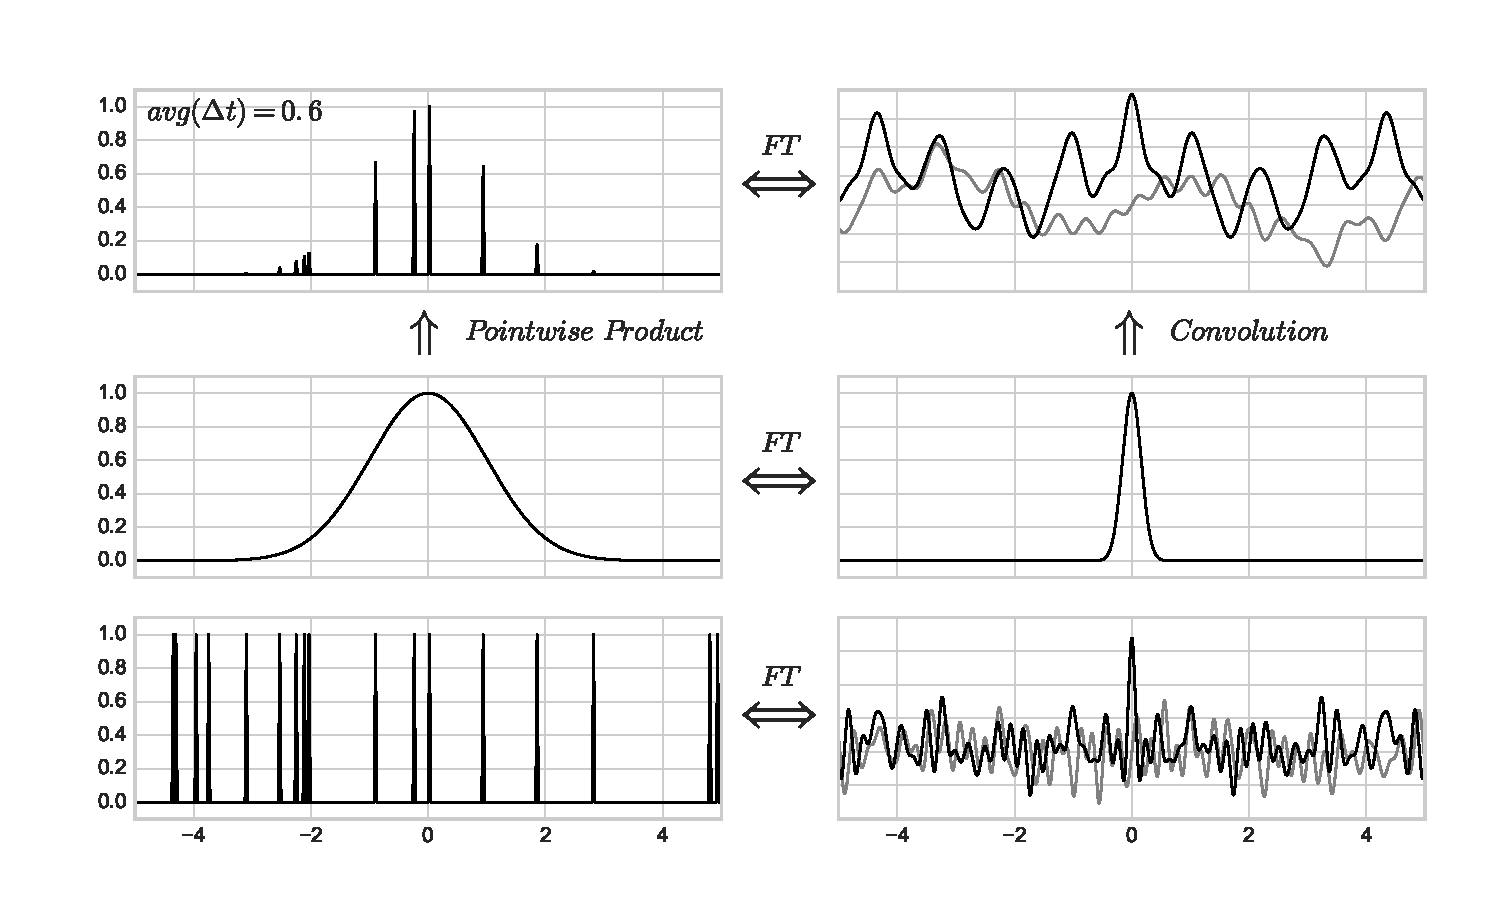
\includegraphics[width=\textwidth]{fig10_random_window}
  \caption{The effect of non-uniform sampling on the observed Fourier transform.
    These samples have the same average spacing as those in \fig{comb-window-1},
    but the lack of structure in observing window translates to a lack of
    structure in its transform, causing the observed transform to be ``noisy''.
    \figlabel{random-window}}
\end{figure}

One might hope that sampling the signal more densely might limit these problems,
and it does, but only to a degree.
\Fig{random-window-2} increases the density of observations by a factor of 10,
such that there are 200 total observations over the length-10 observing window.
The observed Fourier transform in this case is much more reflective of the
underlying signal, but still contains a degree of ``noise'' rooted in the
unstructured nature of the spacing between observations.


\begin{figure}[ht]
  \centering
  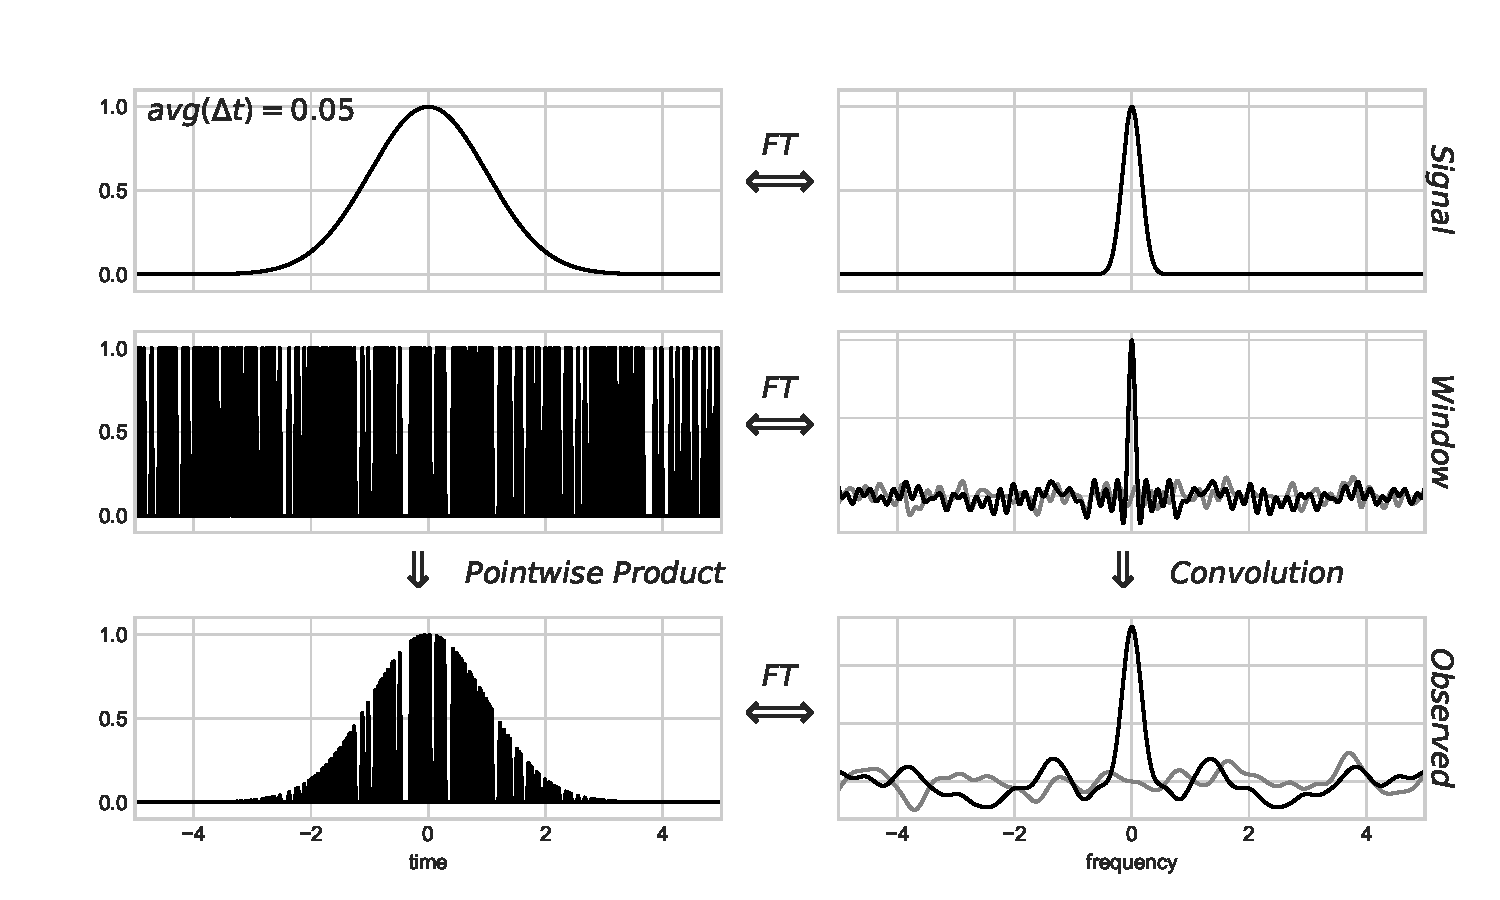
\includegraphics[width=\textwidth]{fig11_random_window_2}
  \caption{The effect of non-uniform sampling on the observed Fourier transform,
    with a factor of 10 more samples than \fig{random-window}.
    Even with very dense sampling of the function, the Fourier transform
    cannot be exactly recovered due to the 
    These samples have the same average spacing as those in \fig{comb-window-1},
    but the lack of structure in observing window translates to a lack of
    structure in its transform, causing the observed transform to be a
    ``noisy'' representation of the true transform
    \figlabel{random-window-2}}
\end{figure}

Since the observed transform is a well-defined convolution of the (unknown) true
transform and the (known) window transform, you might hope that we could
perform some sort of deconvolution operation to recover the result, but this
turns out not to be straightforward, as deconvolution (particularly in this
case where delta functions are involved) is an ill-posed problem without a
unique solution.

\subsection{Non-Uniform Periodogram}

From this non-uniform Fourier transform, it is straightforward to extend the
definition of the Schuster periodogram to the non-uniform case.
Plugging \eq{g-nonuniform} into the Fourier transform of \eq{FT-def}, in analogy to \eq{schuster-periodogram}, gives the following form of the power spectrum:
\begin{equation}
  P(f) = \frac{1}{N}\left|\sum_{n=1}^N g(t_n)e^{-2\pi i t_n} \right|^2
\end{equation}
Becuase it is derived from the Fourier transform of a non-uniformly sampled
function, this periodogram is subject to all the caveats mentioned here: in
particular, the periodogram measures the periodic content of the
{\it windowed signal} and thus reflects a convolution of the true signal
with a non-structured window function.
The resulting periodogram, then, can only be used as a qualitative approximation
of the true periodogram, and will only approach the true periodogram as the
number of observed samples gets very large.


\subsection{A Non-uniform Nyquist Limit?}
\sectlabel{pseudo-nyquist}

As we have seen in \sect{nyquist}, the Nyquist limit is a direct consequence
of the window function created by evenly-sampled data,
and uneven sampling destroys the symmetry that underlies its definition.
Nevertheless, the idea of the ``Nyquist frequency'' seems to have taken hold
in the scientific psyche to the extent that it's often mis-applied in areas
where it is utterly irrelevant.
For unevenly-sampled data, the ``Nyquist limit'' might or might not exist,
and even in cases where it does exist it tends to be far less relevant than
in the evenly-sampled case.

\subsubsection{Incorrect Limits in the Literature}

In the scientific literature, there are countless examples of attempts to
define a ``pseudo-Nyquist'' frequency to apply in the uneven sampling case.
A few common approaches include the mean of the sampling intervals
\citep[e.g.][]{Scargle82, Horne86, NumRec},
the harmonic mean of the sampling intervals \citep[e.g.][]{Debosscher07},
or the minimum sample spacing \citep[e.g.][]{Percy86, Roberts87, Press89, Hilditch01}.
All of these are tempting criteria in that they recover the classical Nyquist 
frequency in the limit of evenly-spaced data, but this does not make up for the
fact that they are wrong.
Several of these cases do parenthetically note that signals at frequencies
beyond the proposed limit are observable in principle, but they nevertheless
proceed under the apparent impression that such pseudo-Nyquist reasoning
is relevant.

As a simple example of where such logic fails,
consider the data from \fig{LINEAR-data}: though the mean sample
spacing is one observation every seven days, in \fig{LINEAR-power}
we were nevertheless able to quite clearly identify a period of 2.58 hours---
an order of magnitude shorter than the mean-based pseudo-Nyquist limit
would indicate as possible.
For the data in \fig{LINEAR-data}, the minimum sample spacing is just under 10
seconds, but it it irresponsible to pretend that this single pair of
observations itself defines some limit beyond which frequency information is
unattainable.

\begin{figure}[ht]
  \centering
  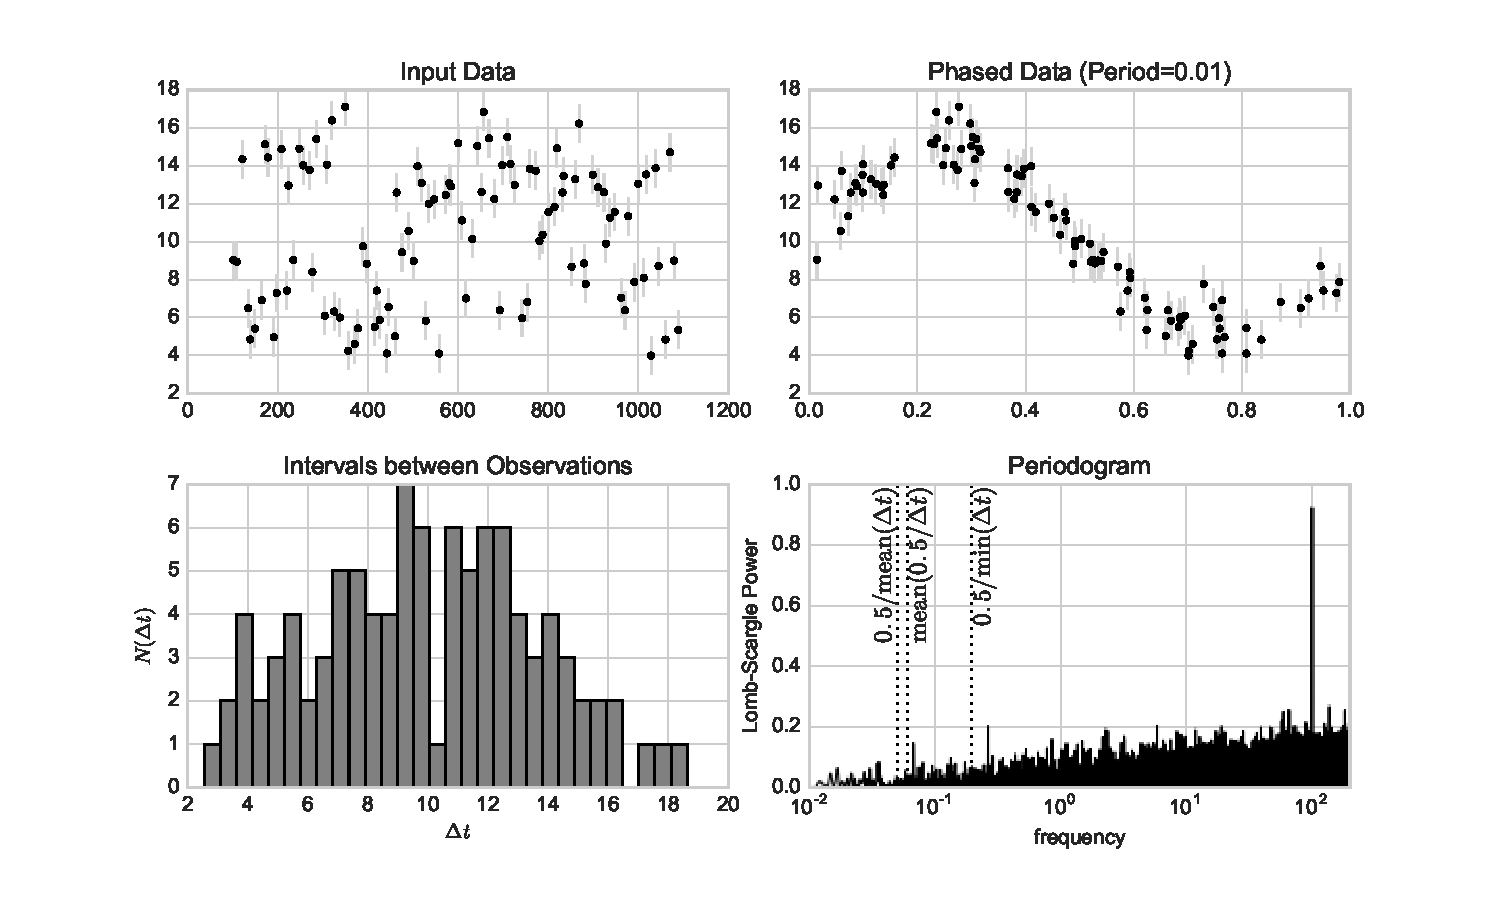
\includegraphics[width=\textwidth]{fig12_pseudo_nyquist}
  \caption{An example of data for which the various poorly-motivated
    ``pseudo-Nyquist'' approaches outlined in \sect{pseudo-nyquist} fail
    spectacularly. The upper panels show the data, a noisy sinusoid with
    a frequency of 100 (i.e. a period of 0.01).
    The lower left panel shows a histogram of spacings between observations:
    the minimum spacing is 2.55, meaning that the signal has
    {\it over 250 full cycles} between the closest pair of observations.
    Nevertheless, the periodogram (lower right) clearly identifies the correct
    period, though it's orders of magnitude larger than pseudo-Nyquist
    estimates based on average or minimum sampling rate.
    \figlabel{pseudo-nyquist}}
\end{figure}

As a more extreme example, consider the data shown in \fig{pseudo-nyquist}.
This consists of noisy samples from a sinusoid with a period of 0.01 units,
with sample spacings ranging between 2 and 18 units: needless to say, any
pseudo-Nyquist definition based on an average or minimum sample spacings
will be {\it far} smaller than the true frequency of 100; still, the
the Lomb-Scargle periodogram in the lower right panel shows quite cleanly
the true frequency.

\subsubsection{The Correct Non-uniform Nyquist Limit}

While Nyquist arguments based on average or minimum sampling fail spectacularly,
there is a sense in which the Nyquist limit can be applied to unevenly-spaced
data. \citet{Eyer99} explores this issue in some detail, and in particular
proves the following:
\begin{quote}
Let $p$ be the largest value such that each $t_i$ can be written $t_i = t_0 + n_i p$, for integers $n_i$. The Nyquist Frequency then is $f_{Ny} = 1 / (2p)$.
\end{quote}
In other words, computing the Nyquist rate for unevenly-spaced data requires
finding some common factor, such that each spacing $\Delta t_i$ is {\it exactly}
an integer multiple of this factor.
This can be proven formally, but can be understood by thinking of such data as
a windowed version of uniformly sampled data with spacing $p$.
Such uniform data has a classical Nyquist limit of $1/(2p)$, and a window function applied to that data cannot change that fact.

\Fig{nyquist-eyer99} shows an example of such a Nyquist frequency.
The data are non-uniformly sampled at times $t_i = n_i * p$, with $p=0.01$.
This results in a Nyquist frequency $f_{Ny} = 50$, and we see the expected
behavior beyond this frequency: the signal at $f > f_{Ny}$ consists of repeated
aliases of the signal at $f < f_{Ny}$.

\begin{figure}[ht]
  \centering
  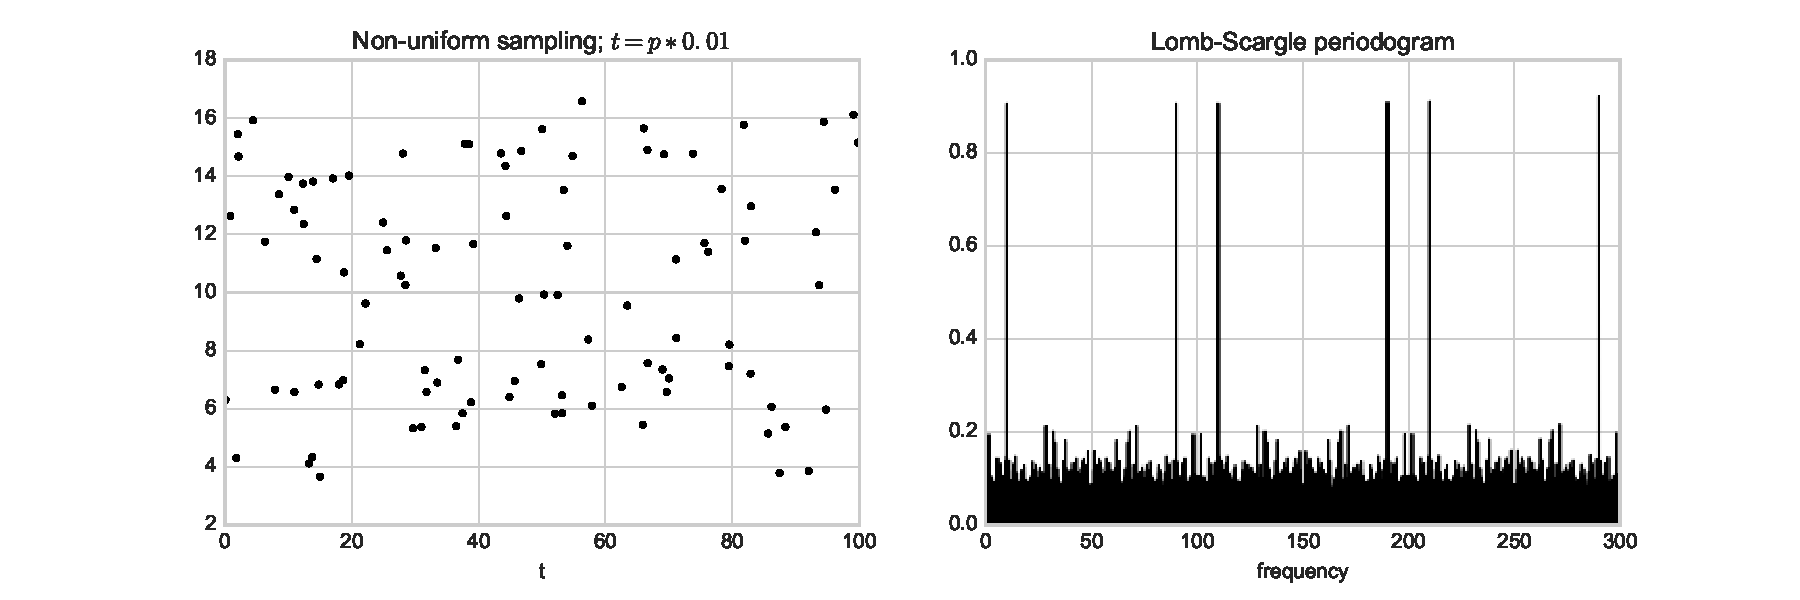
\includegraphics[width=\textwidth]{fig13_nyquist_eyer99}
  \caption{A visualization of the \citep{Eyer99} definition of the Nyquist
    frequency. Data are non-uniformly sampled at times $t_i = n_i p$, for
    integer $n_i$ and $p=0.01$.
    This results in a Nyquist frequency of $f_{Ny}= (2p)^{-1} = 50$:
    the periodogram outside the range $0 \le f < f_{Ny}$ is a series of
    perfect aliases of the signal within that range.
    \figlabel{nyquist-eyer99}}
\end{figure}

We should keep in mind one consequence of this Nyquist definition:
if you have any pair of observation spacings
whose ratio is irrational, {\it the Nyquist limit does not exist!}.
To realize this situation in practice, however, 
requires infinitely precise measurements of the
times $t_i$; more often in the real-world, the Nyquist frequency will be
defined by the precision of the time measurements.
That is, if times are recorded to $D$ decimal places, the Nyquist frequency
will be (at most) $f_{Ny} = \frac{1}{2} 10^D$, as in \fig{nyquist-eyer99}.
In other words, the Nyquist frequency for irregularly-sampled data is most
typically defined by {\it the precision of the time measurements}.

\subsubsection{Limit due to Windowing}

In contexts where observations are not instantaneous, but rather consist of
short-duration integrations of a continuous signal, a qualitatively different
kind of frequency limit exists.
This is typical in, e.g., optical astronomy, where observations take place over
a finite duration $\delta t$.
As noted by \citet{ICVG2014}, this time-scale of integration represents another
kind of limiting frequency for irregularly-sampled data.
Such a situation means that the measurement is effectively a convolution of
the underlying signal with a rectangular window function of width $\delta t$,
in a manner analogous to \fig{convolution-theorem}.
By the convolution theorem, the observed transform will be a point-wise
product between the true transform and the transform of the window, which
will generally have a width proportional to $1/\delta t$.
This means that---absent other more constraining window effects---the
frequency limit is $f_{max} \propto 1/(2\delta t)$, with the constant of
proportionality dependent on the shape of the effective window describing
individual observations.

Keep in mind that the windowing limit $f_{max}$ is quite different than a
Nyquist limit: the Nyquist limit is the frequency beyond which all signal
is aliased into the Nyquist range; the windowing limit is the frequency
beyond which all signal is zero.

\subsection{Semi-structured Observing Windows}

We have seen that for uniform data, the perfect aliasing beyond the Nyquist
frequency is a direct consequence of the symmetry of the Dirac-comb window
function.
For non-uniform observations, such symmetry does not exist, but {\it structure}
in the observing window can lead to partial aliasing of signals in the
data \citep[see, e.g.][]{Deeming75}.


\begin{figure}[ht]
  \centering
  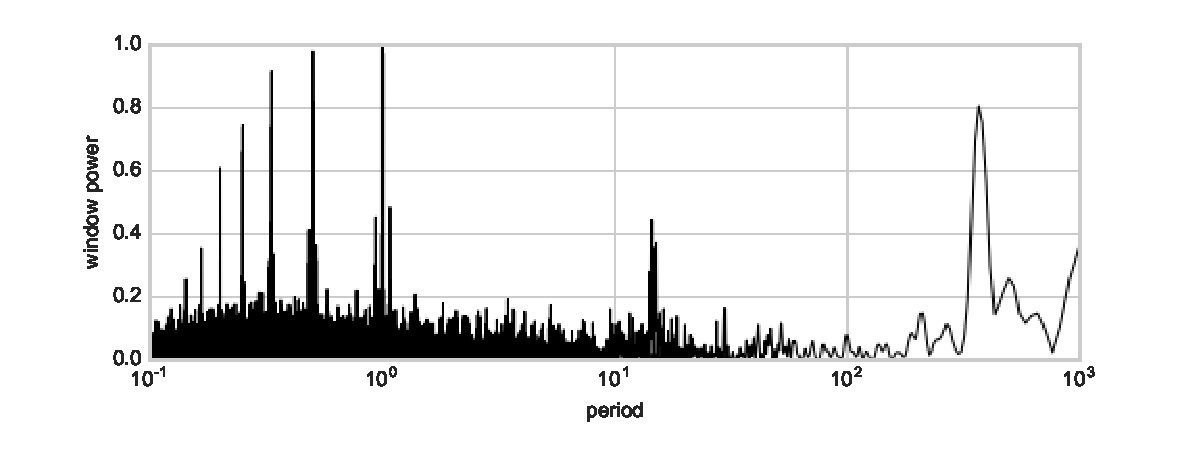
\includegraphics[width=\textwidth]{fig14_LINEAR_window}
  \caption{The power spectrum of the observing window for the data shown
    in \fig{LINEAR-data}. Notice the strong spike in power at a period of
    1 day, and related aliases at $1/n$ days for integer $n$.
    There is also a strong spike at $365$ days, and a noticeable spike at
    $\sim 14$ days. Each of these indicate time intervals that appear often
    in the data.
    \figlabel{LINEAR-window}}
\end{figure}

\subsubsection{A Ground-based Observing Window: LINEAR}

Let's again consider the data shown in \fig{LINEAR-data}. The window power
spectrum for this in \fig{LINEAR-window} shows some quite distinct features,
and these features have an intuitive interpretation.
Namely, if the window power shows a spike at a period of $p$ days, this means
that an observation at time $t_0$ is likely to be followed by another
observation near a time $t_0 + np$ for integer $n$.

Thus the strong spike at a period of 1 day indicate that observations are
taken near the same time of day: this is typical of a ground-based survey
which observes only at night.
The additional spikes at periods of $1/n$ days (for integer $n$) are aliases
of this same effect.

This window also shows a strong spike at a period of 1 year, indicating that
there was a strong seasonal pattern in the observations.
Finally, there is a noticeable spike at approximately 14 days that is likely
related to patterns in scheduling of observing runs.

Recall that a Fourier spectrum observed through a particular window will reflect
a convolution of the true spectrum and the window spectrum
(cf.\ \fig{random-window}), and so we would expect this structure to be
imprinted on the power spectrum measured from the data.


\begin{figure}[ht]
  \centering
  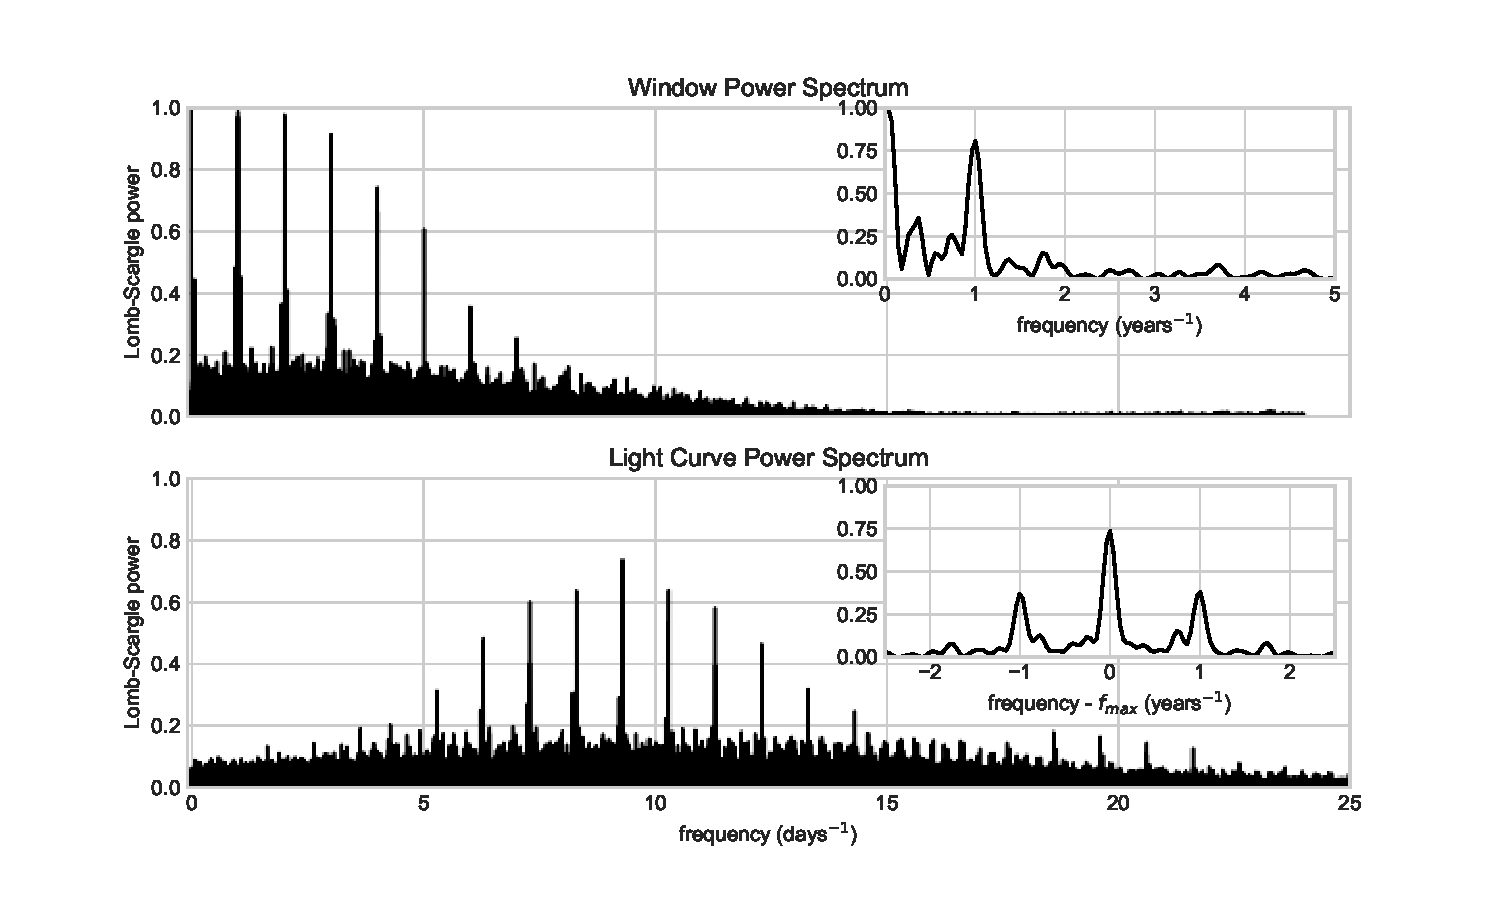
\includegraphics[width=\textwidth]{fig15_LINEAR_window_effect}
  \caption{The effect of the window function in \fig{LINEAR-window} on the
    power spectrum in \fig{LINEAR-power}.
    The top panel shows the window power spectrum, and the bottom panel shows
    the observed signal power spectrum.
    Both are plotted as a function of frequency (we earlier saw both of these
    as a function of period; see \fig{LINEAR-window} and \fig{LINEAR-power},
    respectively).
    Viewing these as a function of frequency makes it clear that the structure
    in the window function is imprinted on the observed spectrum: both the
    diurnal structure in the main panel, and the annual structure in the inset
    are apparent in the observed spectrum.
    \figlabel{LINEAR-window-effect}}
\end{figure}

This behavior is illustrated in \fig{LINEAR-window-effect}.
The upper panel shows the window power spectrum as a function of frequency, while lower panel shows the observed signal power spectrum as a function of frequency.
As noted in the discussion of \fig{LINEAR-window}, the window function shows a strong signal at frequencies corresponding to 1 day and 1 year; the latter can be seen in the inset plot.
The power at both these scales is clearly imprinted on the observed power spectrum, as shown in the lower panel and its inset.
This imperfect aliasing is similar to the perfect aliasing seen in regularly-sampled data at the Nyquist frequency; however, in this case the magnitude of the
aliased signal fades further from the frequency driving the signal.

\subsubsection{A Space-based Observing Window: Kepler}

\begin{figure}[ht]
  \centering
  \includegraphics[width=\textwidth]{fig16_kepler_data}
  \caption{An RR Lyrae variable observed by the Kepler project \citep[see][]{Kolenberg2010}.
    {\it upper left:} the 4083 observed fluxes over roughly three months.
    {\it upper right:} the window power spectrum, which is quite close to that of regularly-spaced data with a cadence of 29.4 minutes.
    {\it lower left:} the time between observations. other than missing measurements, the spacing between observations is nearly uniform. the lower panel gives a closer look at the majority of the spacings, which are not exactly the same but rather span a range of $\pm 50$ms around the mean.
    {\it lower right:} the data power spectrum, showing approximate aliasing and clearly indicating a peak near a period of 13.6 hours, along with higher-order components at multiples of this value.
    \figlabel{kepler-data}}
\end{figure}

Space-based missions often have quite different observing windows.
For example, the upper-left panel of \fig{kepler-data}
shows observations of an RR-Lyrae variable star from the Kepler survey,
measured over 4000 times over a period of three months,
with an irregular observing cadence of just under 30 minutes
 \citep[For deeper discussion of these observations, see][]{Kolenberg2010}.
The Kepler observations are very nearly uniformly-spaced, and this is reflected
in the window power spectrum, shown in the upper-right panel of
\fig{kepler-data}.
The window function is a series of very narrow evenly-spaced spikes,
reminiscent of the Dirac comb shown in \figs{comb-window-1}{comb-window-2},
which we used to motivate the idea of the Nyquist limit.
Thus, in this case we can treat $f_{Ny} = 0.5/29.4$ minutes$^{-1}$ as the
effective Nyquist limit for the data, though aliasing is imperfect due to
the uneven spacing of samples, shown in the lower-left panels of
\fig{kepler-data}.

The lower-right panel of \fig{kepler-data} shows the power spectrum of the
observations, with gray shading indicating the ``Aliased'' region of the
spectrum.
The period of 13.6 hours is strongly apparent, along with smaller spikes at
integer multiples of this frequency that indicate higher-order periodic
components in the signal.

The window functions for ground-based and space-based observations, reflected
by LINEAR data in \fig{LINEAR-window-effect} and Kepler data in
\fig{kepler-data}, are quite different, but in both cases essential features
of the observed power spectra can be understood by recognizing it reflects
not the power spectrum of the underlying signal, but a power specrtrum from
the convolution of the true signal transform and the Fourier transform of
the window function.
For another example of this type of observing window analysis, see
\citep{Deeming75}


\section{From Schuster to Lomb-Scargle}

Up until now, we've been mainly discussing the direct extension of the Schuster
periodogram in \eq{schuster-periodogram} to non-uniform data.
Returning to this definition, we can rewrite the expression in a more
suggestive way:
\begin{eqnarray}
  P(f)
  &=& \frac{1}{N}\left|\sum_{n=1}^N g(t_n)e^{-2\pi i t_n} \right|^2 \nonumber\\
  &=& \frac{1}{N}\left[
    \left(\sum_n g_n \cos(2\pi f t_n)\right)^2
    + \left(\sum_n g_n \sin(2\pi f t_n)\right)^2
    \right]
  \eqlabel{classical-periodogram}
\end{eqnarray}
Although this form of the non-uniform periodogram can be useful for identifying
periodic signals, its statistical properties are not as straightforward as in
the uniform case.
In this case, when we say an estimator with ``good statistical properties'',
we mean that when it is applied to data with straightforward, uncorrelated
noise, the result is a periodogram estimate in which the noise is also
straightforward and uncorrelated.

\citet{Scargle82} showed that while the classical periodogram of
\eq{classical-periodogram} has these desireable statistical properties
in the case of uniform sampling, this does not hold for
\eq{classical-periodogram} when the sampling becomes non-uniform.
To address this, he considered a generalized form of the periodogram,
\begin{equation}
  P(f) = \frac{A^2}{2}\left(\sum_n g_n \cos(2\pi f t_n)\right)^2
       + \frac{B^2}{2} \left(\sum_n g_n \sin(2\pi f t_n)\right)^2,
\end{equation}
where $A$ and $B$ are arbitrary functions of the frequency $f$ and
observing times $\{t_i\}$ (but not the values $\{g_n\}$, and showed
that you can choose one particular form of $A$ and $B$ such that
\begin{itemize}
  \item The periodogram reduces to the classical form in the case of equally-spaced data,
  \item The periodogram has desireable statistical properties, in the sense discussed above,
  \item The periodogram is insensitive to global time-shifts in the data.
\end{itemize}
The values of $A$ and $B$ leading to these properties lead to the following
modification of the classical expression for the periodogram:
\begin{eqnarray}
  P(f) =
  \frac{1}{2} \Bigg\{ &
  \bigg(\sum_n g_n \cos(2\pi f [t_n-\tau])\bigg)^2 \bigg/
  \sum_n \cos^2(2\pi f [t_n-\tau]) &\nonumber\\
  & + ~ \bigg(\sum_n g_n \sin(2\pi f [t_n-\tau])\bigg)^2 \bigg/
  \sum_n \sin^2(2\pi f [t_n-\tau]) & \Bigg\}
  \eqlabel{lomb-scargle-periodogram}
\end{eqnarray}
Here $\tau$ is defined for each $f$ to ensure time-shift invariance of $P(f)$:
\begin{equation}
  \tau = \frac{1}{4\pi f}\tan^{-1}\Bigg(
  \frac{\sum_n \sin(4\pi f t_n)}{\sum_n \cos(4\pi f t_n)}\Bigg).
  \eqlabel{tau-def}
\end{equation}
A remarkable feature of this result is that it is {\it identical} to the result
obtained by fitting a simple sinusoid to the data at each frequency $f$, and
constructing a ``periodogram'' from the $\chi^2$ goodness-of-fit at each
frequency--an estimator which was considered in some depth by \citet{Lomb76}.
Partly due to this deep connection between Fourier analysis and least-squares
analysis, the modified periodogram in \eq{lomb-scargle-periodogram}
has since become commonly referred to as the ``Lomb-Scargle Periodogram''.

Often, the Lomb-Scargle periodogram only differs slightly from the
classical/Schuster periodogram; an example of this is seen in
\fig{ls-comparison}.

\begin{figure}[ht]
  \centering
  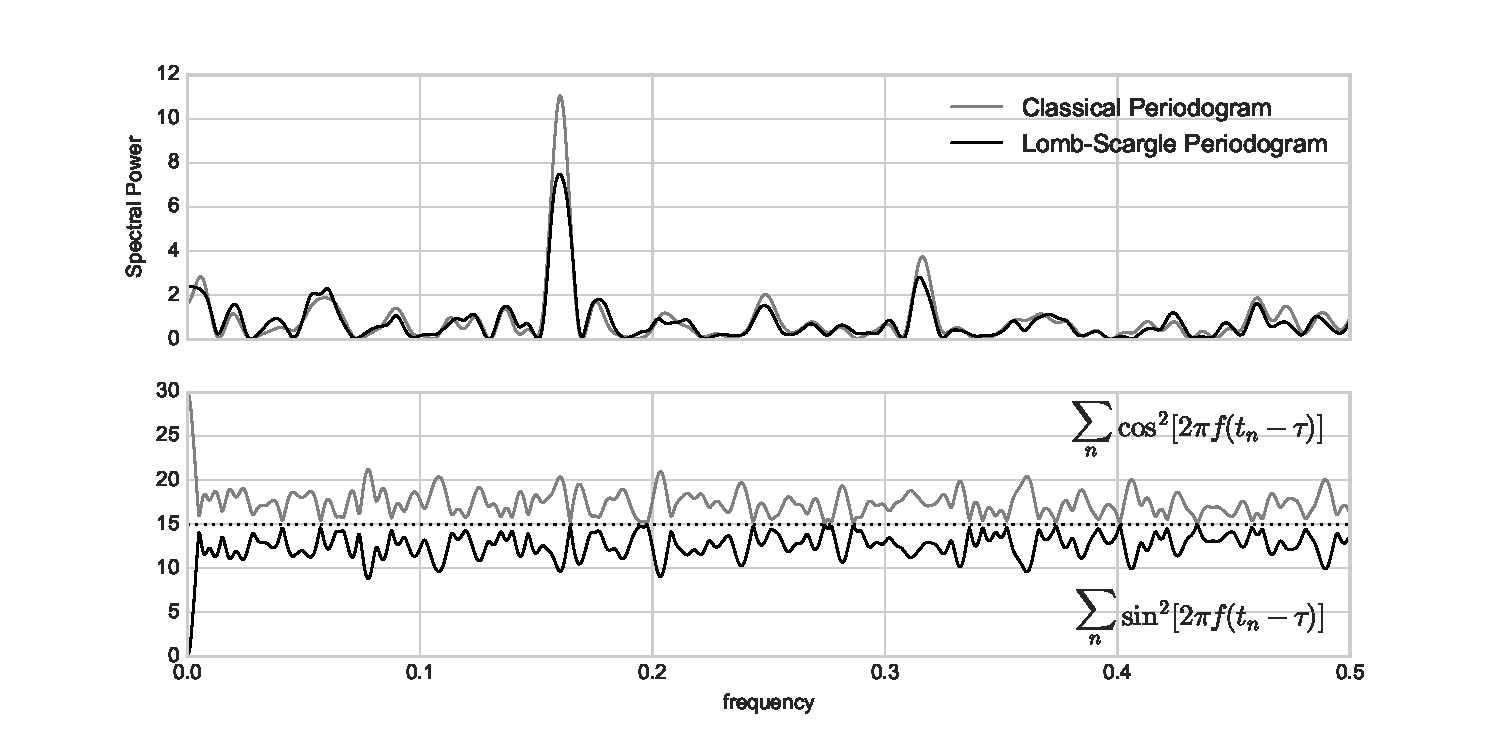
\includegraphics[width=\textwidth]{fig17_ls_comparison}
  \caption{A comparison of the Classical periodogram
    (\eq{classical-periodogram}) and the Lomb-Scargle periodogram
    (\eq{lomb-scargle-periodogram}) for 30 noisy points drawn from a sinusoid.
    Though the two differ quantitatively, the essential qualitative
    features---namely the position of significant peaks---generally remains
    the same.
    \figlabel{ls-comparison}}
\end{figure}

\subsection{Properties of the Lomb-Scargle Periodogram}

\todo{properties of the periodogram}
\begin{itemize}
  \item Reduces to standard form for even spacing
  \item Identical to the $\chi^2$ for a simple sinusoidal fit
    at each frequency
  \item Is qualitatively similar to the classical periodogram, meaning all
    the above discussion is still applicable
\end{itemize}

\todo{show classical vs. lomb-scargle periodogram for LINEAR data}


\section{Using Lomb-Scargle Effectively}

\begin{itemize}
  \item Expected peak width
  \item How to choose the frequency grid
  \item Normalization and interpretation
\end{itemize}


\section{Uncertainties in Periods}

\begin{itemize}
  \item Peak Width and why it's a poor proxy
  \item False Alarm Probability and why it fails
  \item Baluev method and why it's not enough
  \item Motivation of Bootstrap
\end{itemize}



\section{Algorithmic Considerations}

\begin{itemize}
\item Press \& Rybicki method; show some benchmarks.
\item NFFT method
\end{itemize}



\section{Generalizations \& Challenges}

\begin{itemize}
\item Uncertainties in Data
\item Bayesian view is (almost always) not useful
\item Multiterm makes the true period fit better, but also bumps the background noise.
\end{itemize}


\section{Acknowledgements}

\citet{Astropy2013}

\bibliographystyle{apj}
\bibliography{PracticalLombScargle}

\appendix

\section{Non-uniform Nyquist}
A selection of quotations showing approaches to a non-uniform Nyquist limit:

\begin{description}

\item[Average Sampling Rate]

\citet{Scargle82} (citing the following: Beutler 1966, 1970; Masry \& Lui 1975; Higgins 1976; Wiley 1978; Gaster \& Roberts 1975, 1977; Kar, Hornkohl \& Farmer 1981; Ludeman 1981 \todo{read and summarize these!}):
\begin{quote}
Error-free recovery of a band-limited signal [i.e.~reproduction of the entire function $X(t)$ from the samples $X(t_i)$] can be achieved with irregular sampling as long as the mean sampling rate exceeds the Nyquist rate (i.e. the average number of samples per unit time must exceed twice the highest frequency component in the signal).
\end{quote}

\citet{NumRec}: 
\begin{quote}
One guide to choosing $f_{hi}$ is to compare it with the Nyquist frequency $f_c$ which would obtain if the $N$ data points were evenly spaced over the same span $T$, that is $f_c = N/(2T)$. The accompanying program includes an input parameter {\tt hifac}, defined as $f_{hi}/f_{c}$.
\end{quote}

\citet{Horne86}:
\begin{quote}
The largest frequency we calculated was $\pi N/T$ which
is the traditional Nyquist frequency for evenly-spaced data. The Nyquist
frequency is not well defined for unevenly spaced signals, but it can serve as
a reasonable upper limit for the calculation.
\end{quote}

\item[Harmonic Average of Sampling Rate]

\citet{Debosscher07}:
\begin{quote}
For the highest frequency, we used the average of the inverse time intervals
between the measurements: $f_N = 0.5(1/\Delta T)$ as a pseudo
Nyquist frequency. Note that $f_N$ is equal to the Nyquist frequency
in the case of equidistant sampling. For particular cases,
an even higher upper limit can be used \citep[see][]{Eyer99}.
Our upper limit should be seen as a compromise between
the required resolution to allow a good fitting, and computation
time.
\end{quote}


\item[Minimum Sample Spacing]

\citet{Percy86}:
\begin{quote}
... the Nyquist frequency is not well defined for input data obtained at unequally spaced time intervals, the usual case in astronomy \citep{Scargle82}.
Theoretically such a data set contains informatin on the periodicities down to
$\Delta t = \min(t_i - t{i-1})$. In practice, however, a pseudo-Nyquist frequency may be defined by averaging $\Delta t = (t_i - t_{i-1})$, where large, uncharacteristic temporal gaps are avoided. Alternatively, the harmonic mean of all $\Delta t$ may be used. The result is that a useful pseudo-Nyquist frequency may be defined by $\nu_{Ny} = (2 \langle\Delta t \rangle)^{-1}$.
\end{quote}

\citet{Press89}:
\begin{quote}
It is often meaningful to examine frequencies significantly higher than the
Nyquist frequency that would obtain if the same number of data points were
evenly spaced in the same total length of time. Some spectral information is
obtainable for frequencies all the way up to something like half the inverse
spacing of the {\it closest} spaced points.
\end{quote}

\citet{Roberts87}:
\begin{quote}
...for arbitrary $\{t_r\}$, the sampling theorem tells us nothing.
If the data samples are otherwise equally spaced but with missing
points, the theorem says that the data completely determine
a function whose FT is zero for $|v| > 1/(2\Delta_{max})$, where $\Delta_{max}$
is the {\it largest completely sampled} data spacing. However,
there are smaller spacings, and these certainly carry information
about frequencies greater than $1/(2\Delta_{max} )$; some information
is available about frequencies as high as
$1/(2\Delta_{min} )$, where $\Delta_{min}$ is the smallest spacing between data
points. Furthermore, if the $\{t_r\}$ are more or less randomly
distributed, so that a wide range ofspacings are present and
there is little redundancy in the spacing between various
points, tests have shown (Paper II) that significant information
is available on frequencies greater than $l/(2\Delta_{min})$.

Nonetheless, in the present paper we will restrict ourselves
to frequencies obeying
$\nu < \nu_{max} = 1/(2\Delta_{min})$.
\end{quote}

\citet{Hilditch01}:
\begin{quote}
The highest frequency, for equally spaced data, is formally given by the {\it Nyquist frequency}, $f_N = 1/(2\Delta t)$, where $\Delta t$ is the {\it sampling interval} in the data string.
For unequally spaced data, it is common practice to estimate a pseudo-Nyquist frequency from the minimum value of $\Delta t$.
\end{quote}

\item[Getting it Right]

\citet{ICVG2014}:
\begin{quote}
As a good choice for the maximum search frequency, a pseudo-Nyquist frequency $\omega_{max} = \pi/\Delta t$, where $1/\Delta t$ is the median of the inverse time interval between data points, was proposed by \citet{Debosscher07} (in the case of even sampling, $\omega_{max}$ is equal to the Nyquist frequency). In practice, this choice may be a gross underestimate because unevenly sampled data can detect periodicity with frequencies even higher than $2\pi / \Delta t_{min}$ \citep[see][]{Eyer99}. An appropriate choice of $\omega_{max}$ thus depends on sampling (the phase coverage at a given frequency is the relevant quantity) and needs to be carefully chosen: a hard limit on maximum detectable frequency is of course given by the time interval over which individual measurements are performed, such as imaging exposure time.
\end{quote}

\end{description}

\end{document}
